\documentclass[twoside]{book}

% Packages required by doxygen
\usepackage{fixltx2e}
\usepackage{calc}
\usepackage{doxygen}
\usepackage[export]{adjustbox} % also loads graphicx
\usepackage{graphicx}
\usepackage[utf8]{inputenc}
\usepackage{makeidx}
\usepackage{multicol}
\usepackage{multirow}
\PassOptionsToPackage{warn}{textcomp}
\usepackage{textcomp}
\usepackage[nointegrals]{wasysym}
\usepackage[table]{xcolor}

% Font selection
\usepackage[T1]{fontenc}
\usepackage[scaled=.90]{helvet}
\usepackage{courier}
\usepackage{amssymb}
\usepackage{sectsty}
\renewcommand{\familydefault}{\sfdefault}
\allsectionsfont{%
  \fontseries{bc}\selectfont%
  \color{darkgray}%
}
\renewcommand{\DoxyLabelFont}{%
  \fontseries{bc}\selectfont%
  \color{darkgray}%
}
\newcommand{\+}{\discretionary{\mbox{\scriptsize$\hookleftarrow$}}{}{}}

% Page & text layout
\usepackage{geometry}
\geometry{%
  a4paper,%
  top=2.5cm,%
  bottom=2.5cm,%
  left=2.5cm,%
  right=2.5cm%
}
\tolerance=750
\hfuzz=15pt
\hbadness=750
\setlength{\emergencystretch}{15pt}
\setlength{\parindent}{0cm}
\setlength{\parskip}{3ex plus 2ex minus 2ex}
\makeatletter
\renewcommand{\paragraph}{%
  \@startsection{paragraph}{4}{0ex}{-1.0ex}{1.0ex}{%
    \normalfont\normalsize\bfseries\SS@parafont%
  }%
}
\renewcommand{\subparagraph}{%
  \@startsection{subparagraph}{5}{0ex}{-1.0ex}{1.0ex}{%
    \normalfont\normalsize\bfseries\SS@subparafont%
  }%
}
\makeatother

% Headers & footers
\usepackage{fancyhdr}
\pagestyle{fancyplain}
\fancyhead[LE]{\fancyplain{}{\bfseries\thepage}}
\fancyhead[CE]{\fancyplain{}{}}
\fancyhead[RE]{\fancyplain{}{\bfseries\leftmark}}
\fancyhead[LO]{\fancyplain{}{\bfseries\rightmark}}
\fancyhead[CO]{\fancyplain{}{}}
\fancyhead[RO]{\fancyplain{}{\bfseries\thepage}}
\fancyfoot[LE]{\fancyplain{}{}}
\fancyfoot[CE]{\fancyplain{}{}}
\fancyfoot[RE]{\fancyplain{}{\bfseries\scriptsize Generated by Doxygen }}
\fancyfoot[LO]{\fancyplain{}{\bfseries\scriptsize Generated by Doxygen }}
\fancyfoot[CO]{\fancyplain{}{}}
\fancyfoot[RO]{\fancyplain{}{}}
\renewcommand{\footrulewidth}{0.4pt}
\renewcommand{\chaptermark}[1]{%
  \markboth{#1}{}%
}
\renewcommand{\sectionmark}[1]{%
  \markright{\thesection\ #1}%
}

% Indices & bibliography
\usepackage{natbib}
\usepackage[titles]{tocloft}
\setcounter{tocdepth}{3}
\setcounter{secnumdepth}{5}
\makeindex

% Hyperlinks (required, but should be loaded last)
\usepackage{ifpdf}
\ifpdf
  \usepackage[pdftex,pagebackref=true]{hyperref}
\else
  \usepackage[ps2pdf,pagebackref=true]{hyperref}
\fi
\hypersetup{%
  colorlinks=true,%
  linkcolor=blue,%
  citecolor=blue,%
  unicode%
}

% Custom commands
\newcommand{\clearemptydoublepage}{%
  \newpage{\pagestyle{empty}\cleardoublepage}%
}

\usepackage{caption}
\captionsetup{labelsep=space,justification=centering,font={bf},singlelinecheck=off,skip=4pt,position=top}

%===== C O N T E N T S =====

\begin{document}

% Titlepage & ToC
\hypersetup{pageanchor=false,
             bookmarksnumbered=true,
             pdfencoding=unicode
            }
\pagenumbering{alph}
\begin{titlepage}
\vspace*{7cm}
\begin{center}%
{\Large 3D Game Programming Assignment 1 }\\
\vspace*{1cm}
{\large Generated by Doxygen 1.8.12}\\
\end{center}
\end{titlepage}
\clearemptydoublepage
\pagenumbering{roman}
\tableofcontents
\clearemptydoublepage
\pagenumbering{arabic}
\hypersetup{pageanchor=true}

%--- Begin generated contents ---
\chapter{Hierarchical Index}
\section{Class Hierarchy}
This inheritance list is sorted roughly, but not completely, alphabetically\+:\begin{DoxyCompactList}
\item Base\+Application\begin{DoxyCompactList}
\item \contentsline{section}{Basic\+Tutorial2}{\pageref{class_basic_tutorial2}}{}
\end{DoxyCompactList}
\end{DoxyCompactList}

\chapter{Class Index}
\section{Class List}
Here are the classes, structs, unions and interfaces with brief descriptions\+:\begin{DoxyCompactList}
\item\contentsline{section}{\hyperlink{class_basic_tutorial2}{Basic\+Tutorial2} }{\pageref{class_basic_tutorial2}}{}
\end{DoxyCompactList}

\chapter{Class Documentation}
\hypertarget{class_basic_tutorial2}{}\section{Basic\+Tutorial2 Class Reference}
\label{class_basic_tutorial2}\index{Basic\+Tutorial2@{Basic\+Tutorial2}}


{\ttfamily \#include $<$Tutorial\+Application.\+h$>$}

Inheritance diagram for Basic\+Tutorial2\+:\begin{figure}[H]
\begin{center}
\leavevmode
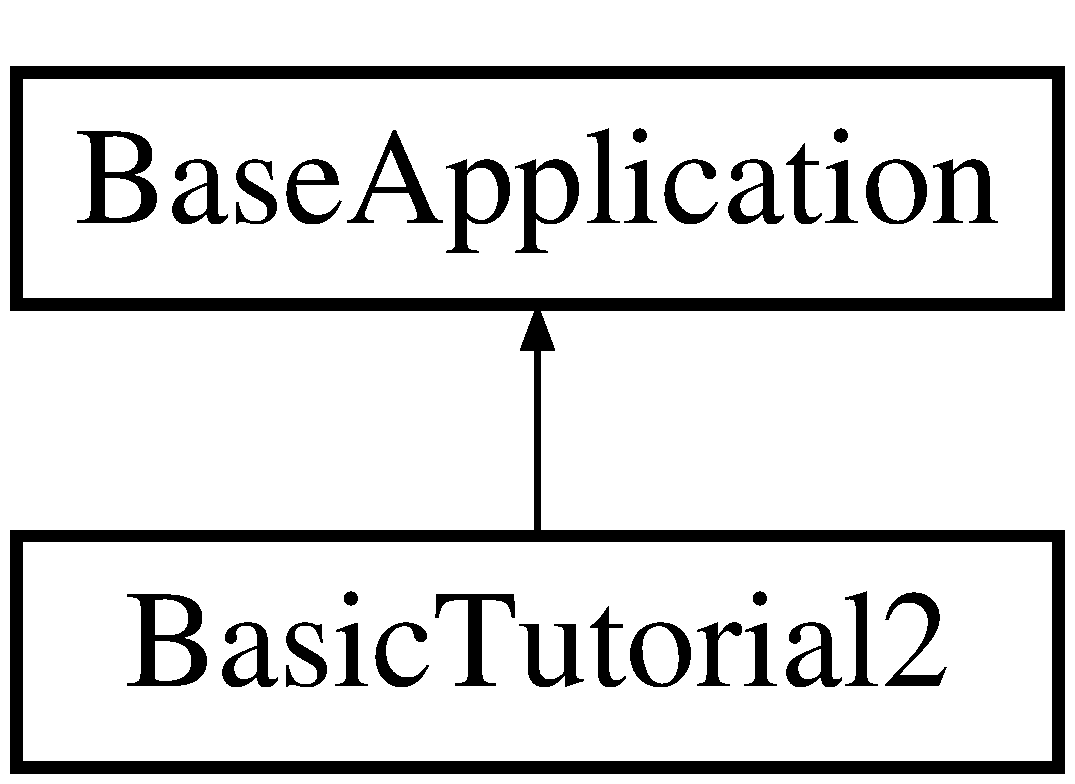
\includegraphics[height=2.000000cm]{class_basic_tutorial2}
\end{center}
\end{figure}
\subsection*{Protected Member Functions}
\begin{DoxyCompactItemize}
\item 
virtual void \hyperlink{class_basic_tutorial2_a4c08f070e21c7cd1f6c415ada8587322}{create\+Scene} (void)
\begin{DoxyCompactList}\small\item\em Create the specific scene. \end{DoxyCompactList}\item 
virtual void \hyperlink{class_basic_tutorial2_affb4d35ed7a64245dec901ae6dbf3497}{create\+Camera} (void)
\begin{DoxyCompactList}\small\item\em Create the camera. \end{DoxyCompactList}\item 
virtual void \hyperlink{class_basic_tutorial2_afb03154c0535bf45f5c3207ddabd4cc5}{create\+Viewports} (void)
\begin{DoxyCompactList}\small\item\em Create the viewports. \end{DoxyCompactList}\item 
virtual void \hyperlink{class_basic_tutorial2_a3074f67362154fce4c99af74c1d7c949}{choose\+Scene\+Manager} (void)
\begin{DoxyCompactList}\small\item\em Choose the scene manager type. \end{DoxyCompactList}\item 
virtual void \hyperlink{class_basic_tutorial2_a633e601ce8a0ac132be83c93ebadb04b}{create\+Circle\+Of\+Objects} (Ogre\+::\+String object\+Mesh, Ogre\+::\+Real num\+Objects, float circle\+Radius, Ogre\+::\+Scene\+Manager $\ast$m\+Scene\+Mgr)
\begin{DoxyCompactList}\small\item\em Create a series of objects that form a circle. \end{DoxyCompactList}\item 
virtual void \hyperlink{class_basic_tutorial2_a92c76d3d02cb8f8fca92ff214bb34139}{create\+Row\+Of\+Objects} (Ogre\+::\+String object\+Mesh, Ogre\+::\+Real num\+Objects, Ogre\+::\+Scene\+Manager $\ast$m\+Scene\+Mgr)
\begin{DoxyCompactList}\small\item\em Create a series of objects that form a row. \end{DoxyCompactList}\item 
virtual void \hyperlink{class_basic_tutorial2_a0b18809c3b7c41ef78f617b3329a6e89}{create\+Default\+Plane} (void)
\begin{DoxyCompactList}\small\item\em Create a plane. \end{DoxyCompactList}\item 
virtual void \hyperlink{class_basic_tutorial2_a04d9c8f1339a0f3e4001a34a48ceef87}{create\+Point\+Light} (Ogre\+::\+String name, Ogre\+::\+Vector3 position, float red\+Value, float green\+Value, float blue\+Value, Ogre\+::\+Scene\+Manager $\ast$m\+Scene\+Mgr)
\begin{DoxyCompactList}\small\item\em Create a point light. \end{DoxyCompactList}\end{DoxyCompactItemize}
\subsection*{Protected Attributes}
\begin{DoxyCompactItemize}
\item 
\hypertarget{class_basic_tutorial2_ae654ab27f10abe32bded5af599ca05ed}{}\label{class_basic_tutorial2_ae654ab27f10abe32bded5af599ca05ed} 
Ogre\+::\+Scene\+Manager $\ast$ {\bfseries m\+Scene\+Mgr0}
\item 
\hypertarget{class_basic_tutorial2_afbf2de4f405faea4abc3914cfad2c081}{}\label{class_basic_tutorial2_afbf2de4f405faea4abc3914cfad2c081} 
Ogre\+::\+Scene\+Manager $\ast$ {\bfseries m\+Scene\+Mgr1}
\end{DoxyCompactItemize}


\subsection{Detailed Description}
Name\+: Zhang Zhexian; ID\+: 0545080; Email\+: \href{mailto:zhangzhexian@outlook.com}{\tt zhangzhexian@outlook.\+com}; 

\subsection{Member Function Documentation}
\hypertarget{class_basic_tutorial2_a3074f67362154fce4c99af74c1d7c949}{}\label{class_basic_tutorial2_a3074f67362154fce4c99af74c1d7c949} 
\index{Basic\+Tutorial2@{Basic\+Tutorial2}!choose\+Scene\+Manager@{choose\+Scene\+Manager}}
\index{choose\+Scene\+Manager@{choose\+Scene\+Manager}!Basic\+Tutorial2@{Basic\+Tutorial2}}
\subsubsection{\texorpdfstring{choose\+Scene\+Manager()}{chooseSceneManager()}}
{\footnotesize\ttfamily void Basic\+Tutorial2\+::choose\+Scene\+Manager (\begin{DoxyParamCaption}\item[{void}]{ }\end{DoxyParamCaption})\hspace{0.3cm}{\ttfamily [protected]}, {\ttfamily [virtual]}}



Choose the scene manager type. 

\begin{DoxyReturn}{Returns}
void 
\end{DoxyReturn}
\hypertarget{class_basic_tutorial2_affb4d35ed7a64245dec901ae6dbf3497}{}\label{class_basic_tutorial2_affb4d35ed7a64245dec901ae6dbf3497} 
\index{Basic\+Tutorial2@{Basic\+Tutorial2}!create\+Camera@{create\+Camera}}
\index{create\+Camera@{create\+Camera}!Basic\+Tutorial2@{Basic\+Tutorial2}}
\subsubsection{\texorpdfstring{create\+Camera()}{createCamera()}}
{\footnotesize\ttfamily void Basic\+Tutorial2\+::create\+Camera (\begin{DoxyParamCaption}\item[{void}]{ }\end{DoxyParamCaption})\hspace{0.3cm}{\ttfamily [protected]}, {\ttfamily [virtual]}}



Create the camera. 

Create the primary and secondary cameras

\begin{DoxyReturn}{Returns}
void 
\end{DoxyReturn}
\hypertarget{class_basic_tutorial2_a633e601ce8a0ac132be83c93ebadb04b}{}\label{class_basic_tutorial2_a633e601ce8a0ac132be83c93ebadb04b} 
\index{Basic\+Tutorial2@{Basic\+Tutorial2}!create\+Circle\+Of\+Objects@{create\+Circle\+Of\+Objects}}
\index{create\+Circle\+Of\+Objects@{create\+Circle\+Of\+Objects}!Basic\+Tutorial2@{Basic\+Tutorial2}}
\subsubsection{\texorpdfstring{create\+Circle\+Of\+Objects()}{createCircleOfObjects()}}
{\footnotesize\ttfamily void Basic\+Tutorial2\+::create\+Circle\+Of\+Objects (\begin{DoxyParamCaption}\item[{Ogre\+::\+String}]{object\+Mesh,  }\item[{Ogre\+::\+Real}]{num\+Objects,  }\item[{float}]{circle\+Radius,  }\item[{Ogre\+::\+Scene\+Manager $\ast$}]{m\+Scene\+Mgr }\end{DoxyParamCaption})\hspace{0.3cm}{\ttfamily [protected]}, {\ttfamily [virtual]}}



Create a series of objects that form a circle. 

A circle is formed by repeatedly rendering the same basic units of objects that are distributed evenly. The objects have varying heights that follow a sine function to produce a wavy effect.


\begin{DoxyParams}{Parameters}
{\em object\+Mesh} & The type of object that forms the circle \\
\hline
{\em num\+Objects} & The number of basic units of objects \\
\hline
{\em circle\+Radius} & The radius of the circle formed by objects \\
\hline
{\em m\+Scene\+Mgr} & The target scene manager\\
\hline
\end{DoxyParams}
\begin{DoxyReturn}{Returns}
void 
\end{DoxyReturn}
\hypertarget{class_basic_tutorial2_a0b18809c3b7c41ef78f617b3329a6e89}{}\label{class_basic_tutorial2_a0b18809c3b7c41ef78f617b3329a6e89} 
\index{Basic\+Tutorial2@{Basic\+Tutorial2}!create\+Default\+Plane@{create\+Default\+Plane}}
\index{create\+Default\+Plane@{create\+Default\+Plane}!Basic\+Tutorial2@{Basic\+Tutorial2}}
\subsubsection{\texorpdfstring{create\+Default\+Plane()}{createDefaultPlane()}}
{\footnotesize\ttfamily void Basic\+Tutorial2\+::create\+Default\+Plane (\begin{DoxyParamCaption}\item[{void}]{ }\end{DoxyParamCaption})\hspace{0.3cm}{\ttfamily [protected]}, {\ttfamily [virtual]}}



Create a plane. 

Create a plane with default settings, which are\+: width 1500, height 1500, x-\/segment 20, y-\/segment 20, number of texture sets 1, x-\/tile 5, y-\/tile 5, upward vector Z axis

\begin{DoxyReturn}{Returns}
void 
\end{DoxyReturn}
\hypertarget{class_basic_tutorial2_a04d9c8f1339a0f3e4001a34a48ceef87}{}\label{class_basic_tutorial2_a04d9c8f1339a0f3e4001a34a48ceef87} 
\index{Basic\+Tutorial2@{Basic\+Tutorial2}!create\+Point\+Light@{create\+Point\+Light}}
\index{create\+Point\+Light@{create\+Point\+Light}!Basic\+Tutorial2@{Basic\+Tutorial2}}
\subsubsection{\texorpdfstring{create\+Point\+Light()}{createPointLight()}}
{\footnotesize\ttfamily void Basic\+Tutorial2\+::create\+Point\+Light (\begin{DoxyParamCaption}\item[{Ogre\+::\+String}]{name,  }\item[{Ogre\+::\+Vector3}]{position,  }\item[{float}]{red\+Value,  }\item[{float}]{green\+Value,  }\item[{float}]{blue\+Value,  }\item[{Ogre\+::\+Scene\+Manager $\ast$}]{m\+Scene\+Mgr }\end{DoxyParamCaption})\hspace{0.3cm}{\ttfamily [protected]}, {\ttfamily [virtual]}}



Create a point light. 

A point light with default setting (type point light) is created with specific parameters


\begin{DoxyParams}{Parameters}
{\em name} & The unique name for the light \\
\hline
{\em position} & The location where the point light shines from \\
\hline
{\em red\+Value} & R in R\+GB value \\
\hline
{\em green\+Value} & B in R\+GB value \\
\hline
{\em blue\+Value} & G in R\+GB value \\
\hline
{\em m\+Scene\+Mgr} & The target scene manager\\
\hline
\end{DoxyParams}
\begin{DoxyReturn}{Returns}
void 
\end{DoxyReturn}
\hypertarget{class_basic_tutorial2_a92c76d3d02cb8f8fca92ff214bb34139}{}\label{class_basic_tutorial2_a92c76d3d02cb8f8fca92ff214bb34139} 
\index{Basic\+Tutorial2@{Basic\+Tutorial2}!create\+Row\+Of\+Objects@{create\+Row\+Of\+Objects}}
\index{create\+Row\+Of\+Objects@{create\+Row\+Of\+Objects}!Basic\+Tutorial2@{Basic\+Tutorial2}}
\subsubsection{\texorpdfstring{create\+Row\+Of\+Objects()}{createRowOfObjects()}}
{\footnotesize\ttfamily void Basic\+Tutorial2\+::create\+Row\+Of\+Objects (\begin{DoxyParamCaption}\item[{Ogre\+::\+String}]{object\+Mesh,  }\item[{Ogre\+::\+Real}]{num\+Objects,  }\item[{Ogre\+::\+Scene\+Manager $\ast$}]{m\+Scene\+Mgr }\end{DoxyParamCaption})\hspace{0.3cm}{\ttfamily [protected]}, {\ttfamily [virtual]}}



Create a series of objects that form a row. 

A row is formed by repeatedly rendering the same basic units of objects that are distributed evenly. The objects have varying heights that follow a cosine function to produce a wavy effect.


\begin{DoxyParams}{Parameters}
{\em object\+Mesh} & The type of object that forms the circle \\
\hline
{\em num\+Objects} & The number of basic units of objects \\
\hline
{\em m\+Scene\+Mgr} & The target scene manager\\
\hline
\end{DoxyParams}
\begin{DoxyReturn}{Returns}
void 
\end{DoxyReturn}
\hypertarget{class_basic_tutorial2_a4c08f070e21c7cd1f6c415ada8587322}{}\label{class_basic_tutorial2_a4c08f070e21c7cd1f6c415ada8587322} 
\index{Basic\+Tutorial2@{Basic\+Tutorial2}!create\+Scene@{create\+Scene}}
\index{create\+Scene@{create\+Scene}!Basic\+Tutorial2@{Basic\+Tutorial2}}
\subsubsection{\texorpdfstring{create\+Scene()}{createScene()}}
{\footnotesize\ttfamily void Basic\+Tutorial2\+::create\+Scene (\begin{DoxyParamCaption}\item[{void}]{ }\end{DoxyParamCaption})\hspace{0.3cm}{\ttfamily [protected]}, {\ttfamily [virtual]}}



Create the specific scene. 

Create the scene of penguins and cube

\begin{DoxyReturn}{Returns}
void 
\end{DoxyReturn}
\hypertarget{class_basic_tutorial2_afb03154c0535bf45f5c3207ddabd4cc5}{}\label{class_basic_tutorial2_afb03154c0535bf45f5c3207ddabd4cc5} 
\index{Basic\+Tutorial2@{Basic\+Tutorial2}!create\+Viewports@{create\+Viewports}}
\index{create\+Viewports@{create\+Viewports}!Basic\+Tutorial2@{Basic\+Tutorial2}}
\subsubsection{\texorpdfstring{create\+Viewports()}{createViewports()}}
{\footnotesize\ttfamily void Basic\+Tutorial2\+::create\+Viewports (\begin{DoxyParamCaption}\item[{void}]{ }\end{DoxyParamCaption})\hspace{0.3cm}{\ttfamily [protected]}, {\ttfamily [virtual]}}



Create the viewports. 

Create the primary and secondary viewports

\begin{DoxyReturn}{Returns}
void 
\end{DoxyReturn}


The documentation for this class was generated from the following files\+:\begin{DoxyCompactItemize}
\item 
source/Tutorial\+Application.\+h\item 
source/Tutorial\+Application.\+cpp\end{DoxyCompactItemize}

%--- End generated contents ---

% Index
\backmatter
\newpage
\phantomsection
\clearemptydoublepage
\addcontentsline{toc}{chapter}{Index}
\printindex

\end{document}
